\documentclass{article}
\usepackage[hmargin={25mm,25mm},vmargin={25mm,25mm}]{geometry} 
\usepackage{parskip}
\usepackage[export]{adjustbox}
\usepackage{graphicx} % Required for inserting images
\usepackage[italicdiff]{physics}
%\usepackage{algorithm}
%\usepackage{algpseudocode}
\usepackage{verbatim}
\usepackage{listings}
\usepackage{xcolor}
\usepackage{filecontents}
\usepackage{subcaption}

\title{C1: Research Computing Coursework Assignment}
\author{Fayzan Mahmood}
\date{December 2024}
\begin{document}

\maketitle
\textit{Remember to add WORDCOUNT and use of AI TOOLS}

\section*{Introduction}
This report details my implementation of a Python package that performs automatic differentiation using dual numbers. A dual number is of the form $a+b\epsilon$, where $a$ and $b$ are real numbers and $\epsilon$ is such that $\epsilon^2=0$ but $\epsilon \neq 0$. The values $a$ and $b$ are referred to as the 'real' and 'dual' parts of a dual number respectively. In this project, I implement a Python class that extends mathematical operations and some common mathematical functions to dual numbers. 

The report will outline the various stages of development of the package. In section 1, I will briefly discuss the initial repository structure. In section 2, I will detail the implementation of the \texttt{Dual} class, how to install the package and how to utilise it to compute derivatives, including an example comparing to the corresponding analytical and numerical results. In section 3, I will discuss my test suite implementation for the package and in section 4 I will cover the Sphinx documentation. Finally, in section 5, I will attempt to Cythonize the package, compare the performance of the Python and Cython versions and build and test Cython wheels.

\section{Initial Repository Structure}

\begin{verbatim}
.
├── tests/
├── docs/
├── dual_autodiff/
│   ├── __init__.py
├── pyproject.toml
├── .gitignore 
└── README.md
        
\end{verbatim}  

My project repository was structured following good practices and initially contained the following files and directories:
\begin{itemize}
    \item \texttt{pyproject.toml} file: To configure the package.
    \item \texttt{dual\_autodiff/} directory: This is where the source code of the package will be located. It must contain an \texttt{\_\_init\_\_.py} file to create a package out of the source code.
    \item \texttt{docs/} directory: Where the documentation will be placed.
    \item \texttt{tests/} directory: Where the test files will be placed to test the package.
    \item \texttt{README.md} file: This provides an overview of the package and instructions on how to install it.
    \item \texttt{.gitignore} file: To ignore unnecessary files so they do not appear in the repository.
\end{itemize}

I also included a blank \texttt{version.py} file in the \texttt{dual\_autodiff} folder to implement automatic versioning and added the relevant lines to

\subsection{Writing Project Configuration}
My pyproject.toml file for this project is shown below:
\lstset{ basicstyle=\ttfamily\footnotesize, backgroundcolor=\color{lightgray!20}, 
frame=single,
breaklines=true,
captionpos=b, 
numbers=left,
stepnumber=1,
language=python } 
% Display the content of pyproject.toml 
\lstinputlisting{pyproject.toml}

The file contains important information to configure the package. Under \texttt{build-system}, there are a list of of build requirements to build the python package and the build-backend. \texttt{setuptools\_scm} is needed for dynamic versioning. 

The \texttt{[project]} section details other information about the project, including the name; version; a short description of the project; where to find the readme file; the minimum Python version required for this package; the author(s) of the package; and some keywords and classifiers which may help users find the package if uploaded to PyPI. 

One of the core features of the package is the implementation of various mathematical functions on dual numbers, which all depend on NumPy. This has therefore been included in the package dependencies.

The final two lines tell the configuration file to find the package in the same directory level that this file is in.

\textbf{ADD CAVEAT ON VERSIONING}

\section{ Creating the \texttt{dual\_autodiff} Package}

\subsection{Implementing the \texttt{Dual} Class}

The package directory contains two files, \texttt{dual.py} and \texttt{autodiff\_tools.py} that contain a \texttt{Dual} class and many member functions that implement dual numbers, define various operations on them and several mathematical functions. 

The class constructor defines a dual number given a real part and dual part. These are assigned as attributes to an instance of the Dual class and can be called from within a Python session, or alternatively using the corresponding member functions which return either the dual part or real part. 

Most of the functions in \texttt{dual.py} are 'magic methods' (defined by the double underline '\_\_') which overload pre-existing operators to allow them to be used for dual numbers. An important method to implement was the \texttt{\_\_repr\_\_} method which defines how dual numbers are displayed in a Python session or notebook. This is to ensure the following output: 

\begin{lstlisting}
>>> from dual_autodiff import Dual
>>> x=Dual(2,1)
>>> x
Dual(real=2, dual=1)
\end{lstlisting}

The other methods extend arithmetic operators, operate-and-assign operators, comparison operators and unary operators (e.g. returning the inverse or negative of a dual number) so that they apply to dual numbers. The details of each method is explained in the package documentation. Considerations were taken to ensure that the arithmetic operators apply to two numbers of type 'Dual' as well as for real numbers (of type 'int' and 'float') to be combined with dual numbers on either the left-hand side or right-hand side. An example of this can be seen in the tutorial notebook.

The \texttt{autodiff\_tools.py} file imports the \texttt{Dual} class from \texttt{dual.py} and defines functions that implement $\sin(x), \cos(x), \tan(x), \ln(x)$ and $\exp(x)$ on dual numbers. Writing these functions in a separate file is a matter of preference - I felt it is better to have these functions separate from the magic commands as further functions can be added to this file without looking through the main file. These functions are then imported into \texttt{dual.py} and assigned as member functions to the \texttt{Dual} class.

As explained in the question paper, for any function $f$ applied to a dual number,
\[
f(a+b\epsilon) = f(a) + b f^\prime (a) \epsilon,
\]
which follows from Taylor's theorem where the higher order terms vanish since $\epsilon^2 =0$. This is used to implement the functions in \texttt{autodiff\_tools}, for example, 
\[
\sin(a+b\epsilon) = \sin(a) + b \cos(a) \epsilon
\]
so that 
\begin{lstlisting}
    >>> x = Dual(2, 1)
    >>> x.sin()
    Dual(real=0.9092974268256817, dual=-0.4161468365471424)
\end{lstlisting}
where $\sin(2)=0.9092...$ and $1*\cos(2)=-0.4161...$.

Docstrings have been provided for the \texttt{Dual} class and its member functions and structured according to best practices (see section \ref{docs}). Where it is necessary, exception handling has been implemented to deal with errors e.g. division-by-zero when inverting a dual number (see section \ref{tests}).

\subsection{ Installing the Package }
I created a virtual environment in which to install the package. To do this, I ran the following commands in the root directory:
\begin{lstlisting}
    python -m venv venvs/c1_cwk
    source venvs/c1_cwk/Scripts/activate
\end{lstlisting}
Then I run the following command to install the \texttt{dual\_autodiff} package:
\begin{lstlisting}
    pip install -e .
\end{lstlisting}
I can then import the package from anywhere by opening a python session and writing
\begin{lstlisting}
    >>> import dual_autodiff as df
    dual_autodiff package version: 0.1.0
\end{lstlisting}
and the version number is displayed to confirm the package has been imported successfully.

\subsection{ Computing Derivatives using the Package } \label{compderivs}

\begin{figure}[h!]
    \centering
    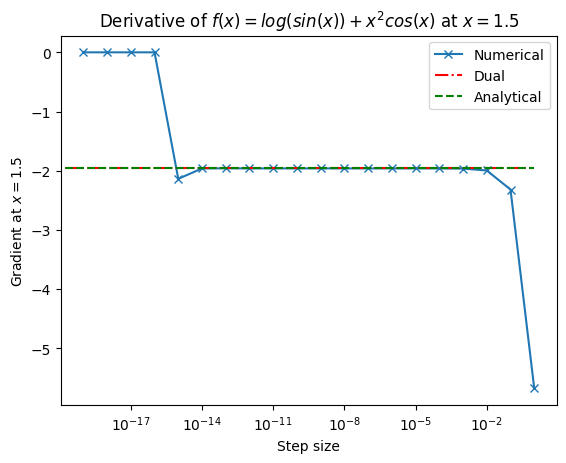
\includegraphics[width=0.7\linewidth]{q5_derivative.png}
    \caption{Derivative of \(f(x) = \log(\sin(x)) +x^2 \cos(x)\) at \(x=1.5\).}
    \label{fig:q5_derivative}
\end{figure}

\begin{figure}[h!]
    \centering
    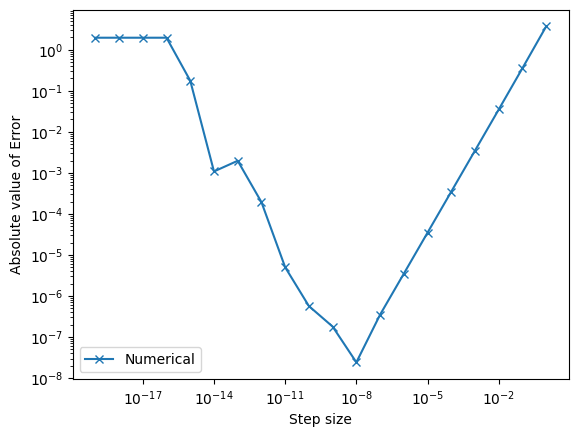
\includegraphics[width=0.7\linewidth]{q5_error.png}
    \caption{Absolute value of error in the numerical derivative of \(f(x) = \log(\sin(x)) +x^2 \cos(x)\) at \(x=1.5\). }
    \label{fig:q5_error}
\end{figure}

The code for this section, including the code to make the plots, can be found in the tutorial notebook \texttt{dual\_autodiff.ipynb}, which is located in the \texttt{docs/Tutorial} directory in the GitLab repository.

As explained earlier, the derivative of any function at $x=a$ can be computed by evaluating the function at $a+\epsilon$ and taking the dual part. Here we evaluate the gradient for the function $ f(x) = \log(\sin(x)) + x^2 \cos(x) $ at $x=1.5$. Computing the derivative using dual numbers and comparing it to the analytical gradient evaluated at the same point, we find that the two results agree up to machine precision (that is, to 16 decimal places). This shows that the dual number method is very accurate, which is highly useful for performing automatic differentiation. This also indicates that the \texttt{Dual} class has been implemented correctly. 

For further comparison, I compute the numerical derivative of the function using a decreasing step size. The result is plotted in Figure \ref{fig:q5_derivative}. This shows that the numerical approximation is quite poor for a step size larger than around $10^{-3}$ (because the higher order terms in the Taylor expansion are not yet small enough) or smaller than around $10^{-15}$ (due to rounding error). From Figure \ref{fig:q5_error}, we also see that at the optimal step size, around $10^{-8}$, the error is still of magnitude $10^{-7}$ which is much larger than machine precision. 

In summary, the numerical derivative is limited by the step size we choose (which is not the case when using dual numbers) and is far less accurate than either the analytical or dual derivative. By contrast, the dual derivative agrees with the analytical one up to machine precision. 

    
\section{Implementing a Test Suite} \label{tests}
The test suite was implemented using \texttt{pytest}. The test files are located in the \texttt{tests} directory in the GitLab repository and contains two test files corresponding to the two modules in the \texttt{dual\_autodiff} directory. I also had to include a blank \texttt{\_\_init\_\_.py} file to remove an error in importing the package when running the tests.

The tests that are implemented \textit{aim} to consider all possible cases in which each method could be used, including invalid uses in particular cases. Tests functions were implemented for every corresponding member function in the \texttt{Dual} class. Test functions of a similar nature were grouped into classes, to help readability. 

For example, to test my overloading of the addition operator, I checked that addition worked in the following cases:
\begin{itemize}
    \item Two dual numbers where the real and dual parts are a mixture of positive and negative integers and floats
    \item Check that adding \texttt{Dual(0,0)} does not change the answer
    \item Adding a dual number and its conjugate (i.e. the conjugate of $a+b\epsilon$ is $a-b\epsilon$) gives the correct result  ($2a+0\epsilon$).
    \item Addition of a real number to a dual on the right
    \item Addition of a real number to a dual on the left
    \item Check that the sum of two real numbers equals a dual number with zero dual part.
\end{itemize}

The above checks were carried out using the \texttt{assert} statement. Other tests involved checking the correct output was displayed, such as when printing an instance of the \texttt{Dual} class, but also in the cases where an error is expected due to an invalid-use case. To do this, I used the pytest functionality \texttt{capsys} to capture the output and an assert statement to check the correct output is shown. Further, in other tests where floating-point precision affects the result, the use of \texttt{pytest.approx} was useful in comparing to the expected outcome to a relevent precision. 

We can then run the test suite with the following command in the root directory:
\begin{lstlisting}
    pytest -s tests/*
\end{lstlisting}
and all of my tests are successful. 

\section{Documentation} \label{docs}
The documentation for this package was created using Sphinx. The docstrings from the \texttt{Dual} class were implemented by linking to the core package modules in the \texttt{*.rst} files and including the \texttt{sphinx.ext.autodoc} extension in the \texttt{conf.py} file, which configures the documentation. The tutorial notebook was also included similarly using the \texttt{nbsphinx} extension. 

The docstrings for the \texttt{Dual} class and its member functions have been formatted as shown in the C1 Research Computing course notes \textbf{REFERENCE} which follows best practices. I have also included some examples in the docstrings for the functions in \texttt{autodiff\_tools}. 

The tutorial notebook showcases some of the various features implemented in the package including all the overloaded operators and mathematical functions. There is also an example which shows how to differentiate the function in section \ref{compderivs} using the \texttt{Dual} class and the same discussion, including the graphs from this section, is included here. There is also a section comparing the performance of the cythonised package, as will be seen in 
the next sections.

Instructions on how to build the documentation are given in the \texttt{README.md} file in the GitLab repository. 

\section{Cythonizing the Package}

\subsection{Creating \texttt{dual\_autodiff\_x}}
\begin{lstlisting}
dual_autodiff_x
├── pyproject.toml
├── requirements.txt
├── setup.py
├── src
   └── dual_autodiff_x
│   │   ├── __init__.py
│   │   └── dual.pyx

\end{lstlisting}

I created a package directory for my Cython package \texttt{dual\_autodiff\_x} as shown above. Initially I wanted to make separate folders for the pure Python package and Cython package, but I had issues with dynamic versioning due to the location of the git tags when I moved the Python package into a subdirectory. Instead I decided to leave my Python package structure as before, with the main \texttt{pyproject.toml} file and make the Cython package directory at the same level. 

Within the \texttt{dual\_autodiff\_x} directory, I added a new \texttt{pyproject.toml} file indicating the location of the new Cython modules and including \texttt{"Cython"} in the build requirements. The \texttt{setup.py} file follows closely the example provided in the C1 notes \textbf{REFERENCE}, which sets up the Cythonized modules/extensions correctly so that we can correctly build the package and wheels.

I copied my Python source code into a single \texttt{dual.pyx} file, as I found it simpler to run in the next section when adding static typing. I then ran the following command
\begin{lstlisting}
    python setup.py build_ext --inplace
\end{lstlisting}
and this created the \texttt{.c} and \texttt{.pyd} files as expected. 

I was then able to install the Cythonized package with \texttt{pip install -e .} from inside the \texttt{dual\_autodiff\_x} directory successfully.

\subsection{ Comparing Performance }

After creating the Cython package, I decided to include static typing in my source code to further optimise the code. The purpose of this is to declare the variable type so that it is known at compile time, removing the need for type checking during execution \textbf{REFERENCE}. Changing the \texttt{def class Dual} to \texttt{cdef class Dual}, or including variable declarations such as \texttt{cdef double real} help are examples of the static typing I included. A consequence of this is that my Cython package can no longer apply the binary operators (e.g. +,-,*,/,+=,...) I defined in the Dual class to a Dual and a non-Dual type (for example, \texttt{Dual(2,1) + 2} is no longer permitted but \texttt{Dual(2,1) + Dual(2,0)} is). Since this would have required redefining many of the functions in my package, I decided to leave this extra functionality out since it is not strictly required for the package to work. 

I compared the performance of both packages in the tutorial notebook by running a set of operations and functions implemented in the packages. I then computed the total time taken to run these tests for different numbers of iterations over 10 calls using the \texttt{timeit} library. The results of this performance comparison are shown in Figure \ref{fig:q9_timeit}. For example, for 100000 iterations I computed an execution time of 13.44 seconds for the Python package compared to 7.55 seconds for the Cython package. From the first graph, we observe that the Cythonized package is slightly faster across different numbers of samples, and is almost twice as fast as is deduced from the second graph. This is due to the fact that the Cython code is compiled in C++, which provides an initial speedup, and static typing which provides an additional speedup. Further optimisation may improve the difference in performance further. \textbf{ADD HERE?}

\begin{figure}
    \centering
    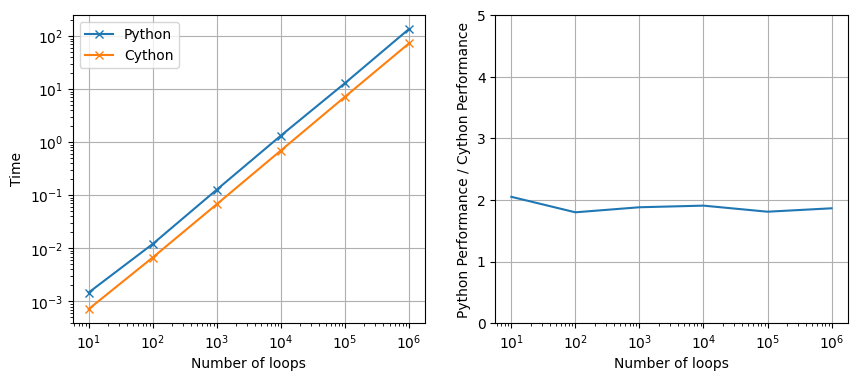
\includegraphics[width=1\linewidth]{q9_timeit.png}
    \caption{Comparing the performance of the pure Python and Cythonized packages.}
    \label{fig:q9_timeit}
\end{figure}

\subsection{Linux Wheels}
To build wheels for the Cythonized package I use \texttt{cibuildwheel} and run Docker on my Windows PC by installing Docker Desktop and opening it. I built Linux wheels for Python 3.11 using the following command given in C1 notes: \textbf{REFERENCE}
\begin{lstlisting}
    CIBW_BUILD="cp311-manylinux_x86_64" CIBW_ARCHS="x86_64" cibuildwheel --platform linux
\end{lstlisting}
 and similarly for Python 3.10 where we change the Python version to \texttt{cp310}. The wheels are located in the \texttt{wheelhouse} directory in the root directory of my Cythonized package. Unzipping the wheels into the \texttt{wheel\_contents} directory, I checked that \texttt{*.pyd, *.so} files and no \texttt{*.pyx} files were present. However, there are still \texttt{*.c} files present and \texttt{\_\_init\_\_.py} files present.

 \subsection{ Using the Linux Wheels }

I now install the package using the wheels I have just created. After uploading the wheels to GitLab and downloading them again, I attempted to install the package on Windows Subsystem for Linux (WSL) on my PC. After creating a virtual environment in the Ubuntu terminal, I was able to install the Python 3.10 wheel successfully using \texttt{pip}. I was then able to run the package in a Python session and import the package in the tutorial notebook (after installing Jupyter with \texttt{pip install Jupyter}). Note that, in order to use the tutorial notebook fully, we also need to install \texttt{numpy, matplotlib} and the \texttt{dual\_autodiff} package as most of the examples are designed for the Python package, not the Cython one. For this reason, I have also created the \texttt{cython\_test} notebook to check that the package runs correctly. 

I also installed the Python 3.11 wheel on CSD3 using the \texttt{scp} command to transfer the downloaded wheel file. The wheel installed successfully and I was able to use the package in a Python session. 

\section*{Summary}

In this project, I have implemented a package that performs automatic differentiation using dual numbers in both Python and Cython. Throughout this project, good software development practices have been demonstrated. I have created a well-structured package; provided a comprehensive and meaningful test suite; and outlined basic usage of the Python package with clear explanations, docstrings and examples in the documentation. I have also successfully Cythonized the package and created Cython wheels for Linux. Finally, I have evaluated the performance of the Cython package and shown that it provides a slight improvement due to static typing and compilation in C. 


\end{document}
